\section{Implementering af database og data-access layer}

\todo{Del evt kode op i mindre dele og forklar alt med henblik på User story vedr. pooldata}

Der er med udgangspunkt i designovervejelserne i afsnit \todo{indsæt reference til design her} implementeret et fungerende data-access layer med tilhørende database.

Dette afsnit vil tage udgangspunkt i to af de væsentligste user stories, \todo{reference til de to user stories}. For dokumentation af resterende user stories, se dokumentationen.

Databasen er implementeret med en Model First tilgang \todo{refence til mf}. Det vil sige at der opsættes en model (ER diagram) for databasen i visual studio, hvorefter der hurtigt kan genereres den samme kode som eller skrives med Code First \todo{reference til CF} tilgangen. Samtidig genereres et SQL script der kan køres mod den specifikke database. Scriptet køres mod en tom database, hvor der ud fra de opstilllede entities genereres tabeller.

Data entiteten som ses på figur~\ref{fig:databaseERD_final_uml} da bruges som en klasse, se klassedigram på figur~\ref{fig:efGeneratedData}. De forskellige datatyper, pH, chlorine, temperature og humidity figurerer som lister (ICollections) i Data klassen. Disse lister er i koden angivet som virtual. Dette er for at gøre lazy loading muligt.

\begin{figure}
\centering
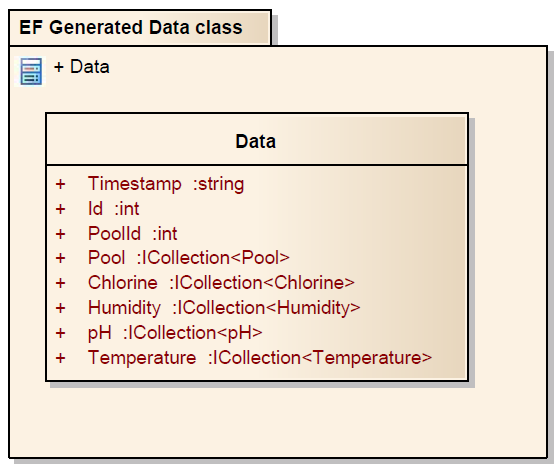
\includegraphics[width=0.5\linewidth]{figs/implementering/efGeneratedData.PNG}
\caption{Data klassen - Genereret fra Entity Model}
\label{fig:efGeneratedData}
\end{figure}


\subsection{Implementering af data-access layer}


\subsubsection{Træk pooldata ud}

\begin{lstlisting}[caption= GetChlorineData method, label=code:getChlorineData]

public List<Tuple<SensorTypes, double>> GetChlorineValues(string poolOwnerEmail, string poolName, int daysToGoBack)
{
double days = System.Convert.ToDouble(daysToGoBack);
string now = DateTime.UtcNow.ToString("G");
string start = DateTime.Parse(now).AddDays(-days).ToString("G");

using (var db = new DatabaseContext())
{   
DateTime startTime = DateTime.ParseExact(start, "dd/MM/yyyy HH:mm:ss", System.Globalization.CultureInfo.InvariantCulture);
DateTime endTime = DateTime.ParseExact(now, "dd/MM/yyyy HH:mm:ss", System.Globalization.CultureInfo.InvariantCulture);

var chlorineDataQuery = from chlorine in db.ChlorineSet
where chlorine.Data.Pool.Name == poolName && chlorine.Data.Pool.User.Email == poolOwnerEmail
select chlorine;

List<Tuple<SensorTypes, double>> chlorineTuples = new List<Tuple<SensorTypes, double>>();

foreach (var chlorine in chlorineDataQuery)
{
if(DateTime.Parse(chlorine.Data.Timestamp).CompareTo(endTime) < 0 ||
DateTime.Parse(chlorine.Data.Timestamp).CompareTo(startTime) > 0)
{
chlorineTuples.Add(new Tuple<SensorTypes, double>(SensorTypes.Chlorine, chlorine.Value));
}
}

return chlorineTuples;
}
}
\end{lstlisting}

\subsubsection{Tilføj user}

\begin{lstlisting}[]
public bool AddUser(string fullname, string email, string password)
{

	if (IsEmailInUse(email)) return false;

	User user;

	if (!ValidateName(fullname)) return false;

	string[] names = fullname.Split(' ');

	if (names.Length <= 2)
	{
		user = new User() { Firstname = names[0], Lastname = names[1], Email = email, Password = password };
	}
	else
	{
		user = new User() { Firstname = names[0], Middelname = names[1], Lastname = names[2], Email = email, Password = password };
	}

	using (var db = new DatabaseContext())
	{
		db.UserSet.Add(user);
		db.SaveChanges();
	}

	return true;
}
\end{lstlisting}





